\documentclass[laboratorio]{guia}

\def \practnum {5} 
\def \practica {Circuito RC}
% \def \practica {Circuito RC: reg\i menes transitorio y estacionario}

\def \materia {Laboratorio de F\'\i sica II para Qu\'\i micos}
\def \periodo {2do. Cuatrimestre de 2015}
\def \catedra {Pablo Cobelli}
\def \website {http://materias.df.uba.ar/f2qa2015c2}
 
\usepackage{graphics}
\usepackage{amsmath}
\usepackage{amsfonts}
\usepackage{graphicx}
\usepackage{float}
\usepackage{wrapfig}
\usepackage{subfigure}
\usepackage{bm}
\usepackage{grffile}
\usepackage{color}
\usepackage{framed}
\usepackage[utf8]{inputenc}
\usepackage[T1]{fontenc}
\usepackage{lmodern}
\usepackage{circuitikz}
\usepackage[spanish]{babel}
\usepackage{babelbib}
\selectbiblanguage{spanish}

 

%----------------------------------------------------------
% Agrega al path de figuras el subdirectorio con el mismo
%     nombre que el archivo principal del proyecto
\graphicspath{{./\jobname/}}

%----------------------------------------------------------
% Definicion del entorno 'sabermas'
\makeatletter
\definecolor{shadecolor}{rgb}{0.89,0.91,0.94}
\newenvironment{sabermas}[1]{%
\vfill
\begin{shaded}
  \begin{center}
  {\textsection{Para saber m\'as}}
  \end{center}
  #1
\sf } 
{%
\end{shaded}%
}
\makeatother

%----------------------------------------------------------
% Definicion del entorno 'problema'
\newcounter{ContadorProblema}
\setcounter{ContadorProblema}{0}
\newcounter{TieneFiguraAsociada}
\setcounter{TieneFiguraAsociada}{0}
\newcounter{UbicacionFigura}
\setcounter{UbicacionFigura}{0}

\newenvironment{problema}[2][]
{%
    \ifx\relax#1\relax%
        \setcounter{TieneFiguraAsociada}{0}
        \else
        \setcounter{TieneFiguraAsociada}{1}
    \fi
    \def \archivofigura {#1}
    % 
    \refstepcounter{ContadorProblema}
    \noindent%
    \ifnum\value{TieneFiguraAsociada} < 1%
        {\sffamily \bfseries Problema \arabic{ContadorProblema}.}
        %{\sc {#1}}%
        \par\nobreak\par\nobreak%
        \medskip 
    \else
        % Va con figura; resta determinar de que lado.
        \ifnum\value{UbicacionFigura} < 1
            % Poner la figura del lado derecho
            \begin{minipage}{12.25cm}
            {\sffamily \bfseries Problema \arabic{ContadorProblema}.}
            %{\sc {#1}}%
            \par\nobreak\par\nobreak%
            \medskip 
        \else
            % Poner la figura del lado izquierdo
            \begin{minipage}{4.5cm}
                \centering
                \includegraphics[width=4.5cm]{\archivofigura}
                {\footnotesize {\sffamily Esquema asociado al 
                problema \arabic{ContadorProblema}}.}
            \end{minipage}\hfill%
            \begin{minipage}{12.25cm}
                {\sffamily \bfseries Problema \arabic{ContadorProblema}.}
                %{\sc {#1}}%
                \par\nobreak\par\nobreak%
                \medskip 
        \fi
    \fi
}
{%
    \ifnum\value{TieneFiguraAsociada} < 1%
        % \par \bigskip \vskip 0.3cm
    \else
        % Va con figura; resta determinar de que lado.
        \ifnum\value{UbicacionFigura} < 1
            % Poner la figura del lado derecho
            \end{minipage}\hfill%
            \begin{minipage}{4.5cm}
                \centering
                \includegraphics[width=4.5cm]{\archivofigura}
                {\footnotesize {\sffamily Esquema asociado al 
                problema \arabic{ContadorProblema}}.}
            \end{minipage}
        \else
            % Poner la figura del lado izquierdo
            \end{minipage}%
        \fi
    \fi
    \setcounter{TieneFiguraAsociada}{0}
    \par \bigskip \vskip 0.3cm
    % Permutamos el valor de la ubicacion
    \ifnum\value{UbicacionFigura} < 1
        \setcounter{UbicacionFigura}{1}
    \else
        \setcounter{UbicacionFigura}{0}
    \fi
}

%----------------------------------------------------------
% Definicion/Redefinicion de estilos
\renewcommand{\vec}[1]{\ensuremath{\mathbf{#1}}}



\hyphenation{ coe-fi-cien-tes coe-fi-cien-te au-to-va-lor
              au-to-va-lo-res co-rres-pon-der pro-ble-ma 
              cual-quie-ra po-la-ri-za-cio-nes }

\graphicspath{{./rc/}}

\begin{document} 
\objetivo{Estudiar los comportamientos de un circuito RC en dos regímenes de operación distintos: transitorio y estacionario.
Para el transitorio, se propone estudiar los procesos de carga y descarga de un capacitor determinando que tipo de evolución temporal presentan, y midiendo los tiempos característicos asociados.
Para el estacionario, se busca determinar la respuesta del circuito al excitarlo con una señal periódica, variando la frecuencia de trabajo del sistema.
    \tematicas{Circuitos de corrientes variables en el tiempo, RC, carga y descarga de un capacitor, tiempo característico, filtros pasa altos y pasa bajos.}
} 
\maketitle


\section{Introducción}
Considere el circuito RC esquematizado en la figura \ref{fig:circuitoRC}, en el cual inicialmente el capacitor se encuentra completamente descargado y el interruptor \(S\) abierta.
Al cerrarse esta ultima, la fuerza electromotriz  \(\varepsilon_0\) impuesta por la fuente genera una corriente \(I\) en el circuito.
Esta corriente tendrá el efecto de llevar cargas de signo opuesto a las caras del capacitor.
Resulta intuitivo que esta corriente no será constante en el tiempo; en particular esperamos que la misma se anule cuando el capacitor se haya cargado.
\begin{figure}[htb]
  \centering
  \begin{circuitikz}
    \draw
      (0,0) to [battery1, l=\(\varepsilon_0\)] (0,1)
      to [closing switch, l=\(S\), o-o] (0,2)
      to [short] (0,2.5)
      to [R, l=\(R\)] (5,2.5)
      to [short] (5,2.5)
      to [capacitor, l=\(C\)] (5,0)
      to [short] (5,0)
      to [short] (0,0)
	  to [short, *-] (0,-0.25)
    ;
    \node[ground]{};
  \end{circuitikz}
  \caption{Esquema del circuito RC empleado.}
  \label{fig:circuitoRC}
\end{figure}


%\begin{figure}[htb]
%  \centering
%  \begin{tikzpicture}
%    % -- Circuito RC -- %
%    \draw[step=0.5, very thin, black!20] (-1, -0.5) grid (6, 2.5);
%    \path (0, 0) coordinate (ref_gnd);
%    \draw
%      (ref_gnd) to[battery1=\(V\)] ++(0,2)
%                    to[R=\(R\)] ++(3,0) 
%                    to[C=\(C\)] ++(0,-2) 
%          -- (ref_gnd);
%  \end{tikzpicture}
%  \vspace{0.5cm}
%  \caption{Esquema del circuito RC empleado.}
%  \label{fig:circuitoRC}
%\end{figure}

% \begin{figure}[t!]
%     \centering
%     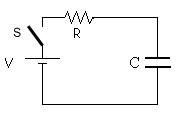
\includegraphics[width=6cm]{LG05--000.png}
%     \caption{Esquema del circuito RC empleado.}
%     \label{fig:circuitoRC}
% \end{figure}



Un capacitor de capacidad \(C\) conectado a una fuente que lo somete a una $\Delta V$ constante adquiere una carga $q = C \Delta V$.
% Esto nos permite conocer la caída de potencial sobre nuestro capacitor.
% Por otro lado, la ecuacion circuital para el circuito RC resulta simplemente:
Por tanto y de acuerdo a la primer ley de Kirchhoff
\begin{equation}
    \varepsilon_0 = RI(t) + \frac{q(t)}{C},
\end{equation}
donde  \(I(t)\) como \(q(t)\) denotan que estas varían instante a instante.
Recordemos, por otro lado, que tanto la $\varepsilon_0$ de la fuente, la resistencia \(R\) del resistor y $C$ son constantes.
Empleando ahora la definición de corriente,
\begin{equation}
  I = \dv{q}{t},
  % I = \frac{dq}{dt},
  \label{corriente}
\end{equation}
podemos reescribir la ultima ecuación en término de una única función incógnita, ya sea \(q(t)\) o \(I(t)\).
Vamos a elegir expresarla en función de \(q(t)\), de lo que se obtiene
\begin{equation}
    \varepsilon_0 = R \dv{q}{t}(t) + \frac{1}{C} q(t).
    \label{eq:ecuacionRC}
\end{equation}
Esta es una ecuación diferencial ordinaria de orden 1 para \(q(t)\), cuya solución nos dará la evolución temporal (desde un instante inicial dado) de la carga en el capacitor. 
Para resolverla, debemos especificar además una condición inicial para la carga \(q(t)\) en el capacitor.
Dado que estamos considerando el caso en el que el mismo se encuentra inicialmente descargado, esta condición es
\begin{equation}
    q(t=0) = 0.
\end{equation}
La ecuación diferencial en derivadas totales para \(q(t)\) dada por
\eqref{eq:ecuacionRC} tiene una solución general de la forma:
\begin{equation}
    q(t) = A \text{e}^{-t/\tau} + C \varepsilon_0,
\end{equation}
donde \(\tau = RC\) es el tiempo característico del circuito RC, y la constante \(A\) se determina de las condiciones del problema particular que se este considerando.
Por ejemplo, si el capacitor esta inicialmente descargado, resulta fácil obtener que \(A = -C \varepsilon_0\), por lo que
\begin{equation}
    q(t) = C \varepsilon_0 \left(1 - \text{e}^{-t/\tau} \right),
\end{equation}
y entonces la corriente en función del tiempo resulta
\begin{equation}
    I(t) = \frac{\varepsilon_0}{R} \text{e}^{-t/\tau}.
\end{equation}

En base a esto, plantee como serían las ecuaciones que describen la
descarga del capacitor, reemplazando para ello la fuente por un cortocircuito.


\section{Carga y descarga de un capacitor}
% En esta primera etapa se estudia el proceso de carga y descarga del capacitor. 
%
%\subsection{Midiendo en forma manual con multímetro}
%
%De realizar la experiencia con cronometro, se sugiere elegir valores de $R$ y
%$C$ de manera tal que el producto $RC$ sea igual o superior a 100 segundos. De
%esta forma los procesos de carga y descarga son lo sufientemente lentos como
%para poder tomar los datos manualmente. 
%
%\subsection{Midiendo a traves de la placa de adquisicion SensorDAQ}
%
%En cualquiera de las dos modalidades que se elija medir, se busca responder
%las siguientes preguntas:

Para realizar la práctica reemplazará en la figura \ref{fig:circuitoRC} a la fuente y el interruptor con un generador de señales.
Utilizará el modo en que este provee una \(\varepsilon_0\) de forma cuadrada.
Como buscamos que la señal tenga siempre la misma polaridad (siempre positiva o siempre negativa) ajustará el \emph{offset} para que la bases (o mesetas) coincidan con el potencial de tierra.
De esta forma simularemos el efecto de abrir y cerrar el circuito en forma periódica con el interruptor.

Para medir diferencias de potencial utilizará un osciloscopio de dos canales.
En el primer canal observará la señal del generador para lo que necesitará conectar a la salida del mismo una \emph{T de BNC} para derivar un cable hacia una entrada del osciloscopio y otro hacia la resistencia.
En el segundo canal del osciloscopio medirá la caída de potencial en el capacitor.
Ajuste ahora en el osciloscopio los niveles de base de ambos canales para que sean coincidentes en la pantalla y sea evidente la superposición de ambas diferencias de potencial, la del generador y la que se registra en el capacitor.

Ajuste la frecuencia hasta que sea evidente la diferencia entre ambas señales, y responda:
\begin{itemize}
  \item ¿Cuál es el tiempo característico (de carga y descarga) que se obtiene de las  mediciones?
  ¿Es el mismo para ambos procesos?
  \item ¿Cuál es el valor de diferencia de potencial que se alcanza al llegar al régimen estacionario? 
  \item ¿En el proceso de descarga, sobre que elemento disipativo se descarga el capacitor?
  \item ¿Es posible estimar la resistencia interna del multímetro? 
\end{itemize}
Repita las mediciones utilizando otro valor de \(\Delta V\) para la fuente.
¿Observa cambios en el tiempo característico producto de esta modificación?


\section{Integrador | Derivador}
Según la expresión (\ref{corriente}) la carga en el capacitor es \(q= \int I \dd{t}\), por lo que la diferencia de potencial sobre este es \(\Delta V_C= C \int I \dd{t}\).
Así midiendo esta \(\Delta V_C\) puede obtener una integración de \(I\).

Se propone ensayar esto alimentando al circuito de la figura \ref{fig:circuitoRC} una señal cuadrada cuya base coincida con \(\Delta V= 0\).
Observe esta señal en un canal del osciloscopio, y en el otro ver la \(\Delta V_C\) en el capacitor.
Superponga ambas señales en la pantalla y ensaye frecuencias relativamente altas (\(f\gg \frac{1}{\tau}\)) hasta observar claramente la señal integrada.
Recordando que el área bajo una función es la integral, verifique que el valor pico de la señal integrada se corresponde con el área de uno de los ciclos de la señal cuadrada.
% Como el área bajo una función es la integral verifique que el área...

Se propone ahora que modifique la conexión para armar el circuito propuesto en la figura \ref{fig:derivadorRC}.
\begin{figure}[htb]
  \centering
  \begin{circuitikz}
    \draw
      (0,0) to [battery1, l=\(\varepsilon_0\)] (0,1.5)
      to [short] (0,1.5)
      to [capacitor, l=\(C\)] (3,1.5)
      to [short] (3,1.5)
      to [R, l=\(R\)] (3,0)
      to [short] (4,0)
      to [short] (0,0)
	  to [short, *-] (0,-0.25)
      (3,1.5) to [short, *-o] (5,1.5) 
      (3,0) to [short, *-o] (5,0)
      (5,0) node[above=15]{\(\Delta V_R\)} 
    ;
    \node[ground]{};
  \end{circuitikz}
  \caption{Esquema de un circuito RC empleado como derivador.}
  \label{fig:derivadorRC}
\end{figure}
Ahora se propone medir en el segundo canal del osciloscopio la caída de potencial en la resistencia que como sabemos responde a la corriente \(\Delta V_R= I R\).
Nuevamente gracias a la expresión (\ref{corriente}) podemos relacionar esta última con la carga del capacitor para obtener que
\begin{equation}
  \Delta V_R= R \dv{q}{t}= R \dv{C \Delta V_C}{t}.
\end{equation}
Y si la frecuencia es lo suficientemente baja \(f \ll \frac{1}{\tau}\)) como para que la \(\Delta V_C\) no se aparte mucho de la \(\varepsilon_0\) que entrega la fuente, tenemos una forma de derivar la señal que entregamos al circuito.

Alimente al circuito \ref{fig:derivadorRC} una señal triangular y ensaye frecuencias bajas hasta observar superpuesta en el osciloscopio la derivada de esta señal.
Como la derivada de una función en cada punto es su pendiente verifique que el valor que puede medir en el segundo canal del osciloscopio se corresponde con el que puede calcular en la señal de entrada.


% \section{Respuesta estacionaria}
% En esta parte de la practica la forma de la señal será sinusoidal, y se variará la frecuencia de esta.

%\subsection{Filtro pasa bajos \ circuito integrador}
%Para esta instancia se sugieren elegir valores de \(R\) y \(C\) de manera que su producto sea del orden de \SI{100}{\micro\second}.
%Aplicando una señal sinusoidal de amplitud de \SI{5}{\volt}, estudie la respuesta del sistema en función de la frecuencia. 
%
%A continuación cambie la forma de onda de la señal de entrada a una onda cuadrada.
%Nuevamente, estudie la forma de la señal de salida en función de la \(f\).
%¿Existe alguna relación entre ambas?
%Intente describir mediante los modelos propuestos los resultados experimentales 
%obtenidos. 
%
%Grafique luego el cociente entre las amplitudes de la señal de salida y la de entrada como función de la frecuencia \(f\).% $f = \omega/(2\pi)$.
%Intente determinar el desfasaje $\phi$ entre la señal de entrada y la de salida; que 
%puede definirse como $\Delta \phi = \omega \Delta t$.
%Estudie como varía este desfasaje en función de la \(f\).%frecuencia.% $f$. 
%
%
%
%\subsection{Filtro pasa altos \ circuito derivador}
%
%Repita las mediciones tomadas en el caso anterior, pero esta vez midiendo 
%la caída de potencial sobre el resistor. 
%Discuta las similitudes y diferencias. 

\nocite{Alonso1998,Purcell1988,Reitz1996,Trelles1984,Reitz1996}
\bibliographystyle{unsrt} 
\bibliography{Bibliografia}

\end{document}
